\section{Impact Analysis}
\subsection{Brief Introduction}
The impact analysis is used to understand the implications of changing a specific feature within the \textit{JHotDraw} project.
The project itself will receive the different feature changes at different times, as the development team, consisting of 5 members,
they are all working on different features of the application at their own pace, and some members might be further ahead than others at any given time.
After inserting the feature entry points into the \textit{JHotDraw} project, I was able to get an output of different relevant figures: \textit{Feature-code Characterization,}
\textit{Feature-code Correlation Grid,} and \textit{Feature-Package Correlation Graph.}

The feature entry points I used in this project are the following:
\begin{itemize}
    \item \textit{Tools-display}
    \item \textit{Drag-drop}
          \begin{itemize}
              \item \textit{Pressed}
              \item \textit{Dragged}
              \item \textit{Released}
          \end{itemize}
\end{itemize}

The \textit{}Tools-display, as stated in the \textit{}Concept Location chapter, is a class that references the \textit{JDisclosureToolbar} class. The \textit{Tools-display} is a handler callback that has been added to a button;
when pressed, it will change the visibility of the chosen toolbar section from visible to hidden or vice versa.

The \textit{Drag-drop}, which consists of \textit{Pressed}, \textit{Dragged}, and \textit{Released}, are handlers that are connected with the \textit{PaletteToolbarUI}. They are activated in the following order:
\begin{itemize}
    \item \textit{Pressed}: when a tool is pressed on with the click of a mouse.
    \item \textit{Dragged}: when a tool has been pressed and the mouse moves while the button is still being held down by the user.
    \item \textit{Released}: when the user releases the pressed mouse button again.
\end{itemize}

\subsection{Featureous Feature-code Characterization}

\begin{figure}[H]
    \centering
    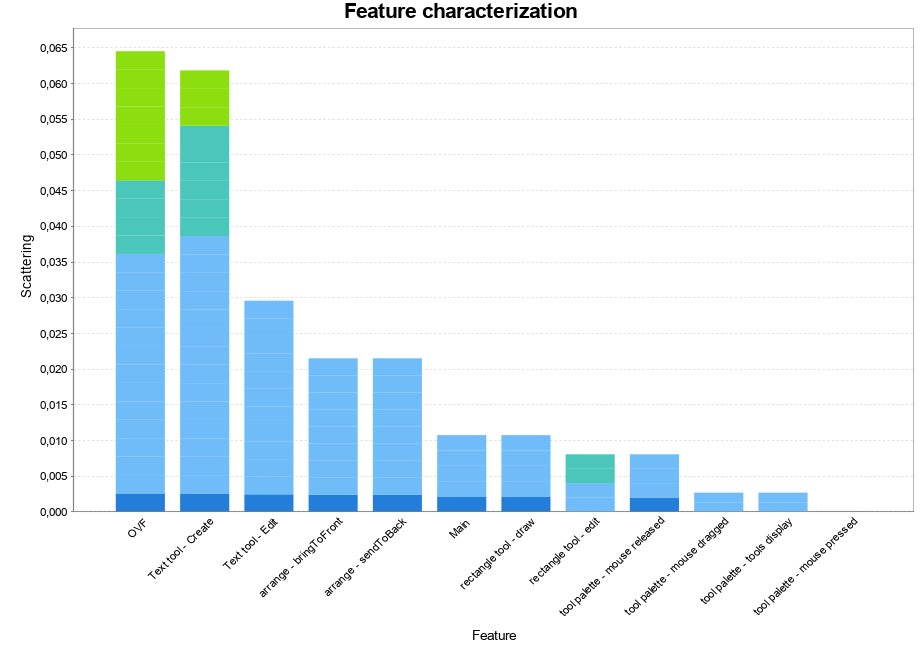
\includegraphics[width=\linewidth]{pic/Featureous Feature-Code Characterization new.png}
    \caption{Featureous Feature-Code Characterization}
    \label{fig:Featureous Feature-Code Characterization}
\end{figure}

As we can see, the units do contain alot of inter-group units, this can if one is not careful, end in entanglement with the other units that other developers
are using in their part of the project, but it does offer us some insights for future refactorings.

\subsection{Featureous Feature Relations Characterization}

\begin{figure}[H]
    \centering
    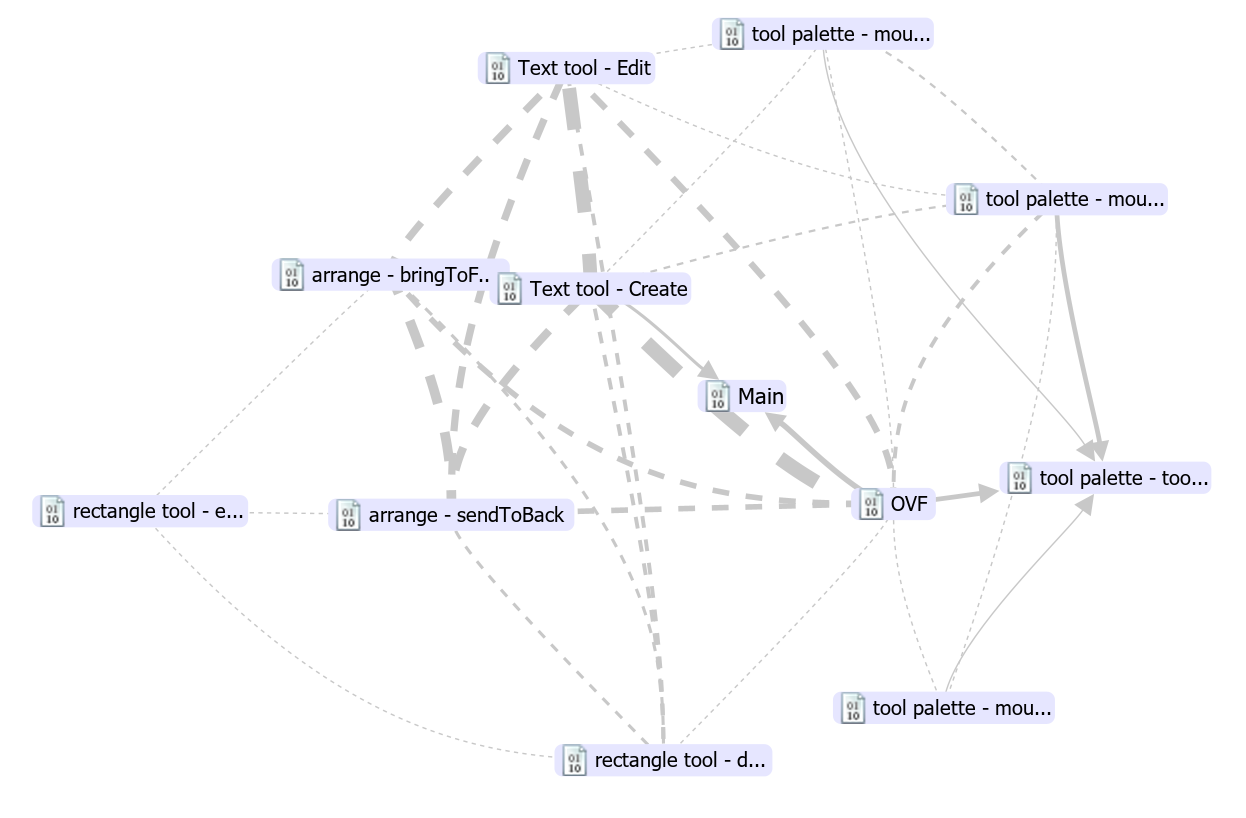
\includegraphics[width=\linewidth]{pic/Feature Relations Characterization new.png}
    \caption{Featureous Feature Relations Characterization}
    \label{fig:Featureous Feature Relations Characterization}
\end{figure}

As one can see, the connections which the entry points have made, does not contain strong connections
with the other features that are also in this project. it does not look like they even engage in any consumer/producer connections.

\subsection{Feature-code correlation graph and feature-code correlation grid}

\begin{figure}[H]
    \centering
    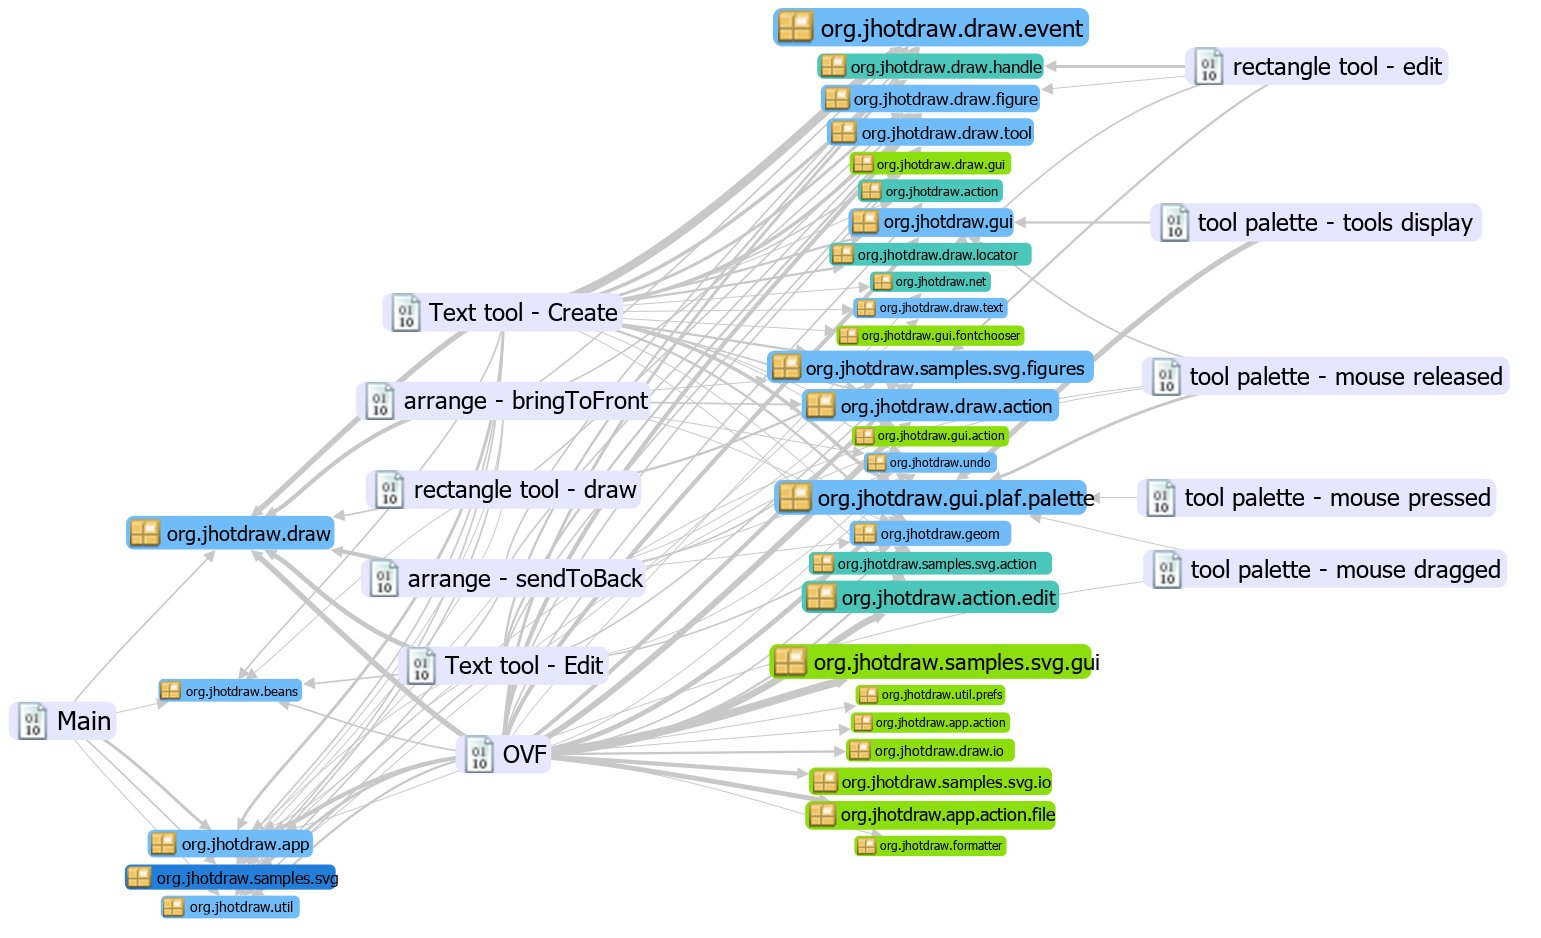
\includegraphics[width=\linewidth]{pic/Feature-Package Correlation Graph new.png}
    \caption{Feature-Package Correlation Graph}
    \label{fig:Feature-Package Correlation Graph}
\end{figure}

These tools can provide a deeper look into the connections between source code units and features,
highlighting relationships and dependencies important for understanding the overall impact of the change request.

But however the \textit{Feature-Package Correlation Graph} does not give the best overview of the connections between the features and the packages.
What it can provide however, is a visual confirmation that there is no strong connections between the \textit{Tool Palette} and the other entry points in the project.



\begin{figure}[H]
    \centering
    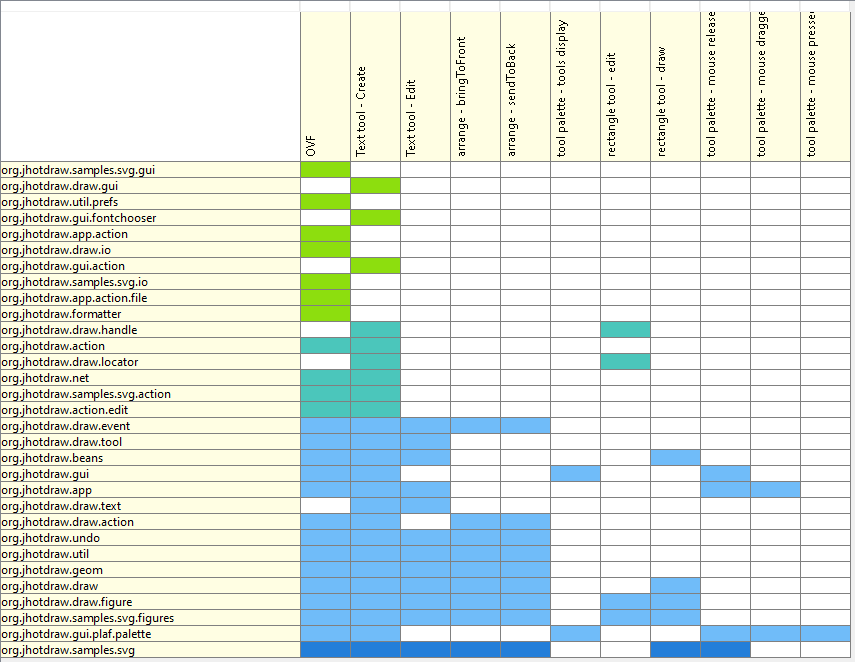
\includegraphics[width=\linewidth]{pic/Feature-Code Correlation Grid new.png}
    \caption{Feature-Code Correlation Grid}
    \label{fig:Feature-Code Correlation Grid}
\end{figure}

The analysis reveals only a small entanglement between my own features and those being used by other developers in the project.



The \textit{drag-drop-released} feature \textit{(mouse released, mouse dragged, mouse pressed)} only connected to the \textit{OVF} package.
The \textit{tools-display} feature also only cross with intergroup packages and the \textit{OVF} package.
For my own features, they are not connected to any other features, meaning that they are not dependent on any other features in the project,
and therefore can be refactored without any worries of breaking other features.
Normally interlinked nature of features requires very careful mindsets of other developers' work before proceeding with development and refactoring of
their parts of the project, but as stated before my own feature does not seem to requires the same deep of a careful mindset when it comes to its refactoring.

\subsection{Table - Impact Analysis}

\begin{table}[H]
    \centering
    \begin{tabular}{|l|c|l|p{5cm}|}
        \hline
        \textbf{\textit{Package name}} & \textbf{\# of classes} & \textbf{Tool used} & \textbf{Comments} \\ \hline
        \textit{.gui}                  & 76                     & Correlation grid   & changed           \\ \hline
        \textit{.gui.plaf.pallete}     & 38                     & Correlation grid   & changed           \\ \hline
        \textit{.samples.svg}          & 65                     & Correlation grid   & unchanged         \\ \hline
        \textit{.draw.event}           & 20                     & Correlation grid   & unchanged         \\ \hline
        \textit{.app}                  & 39                     & Correlation grid   & unchanged         \\ \hline
        \textit{.draw.gui}             & 6                      & Correlation grid   & unchanged         \\ \hline
    \end{tabular}
    \caption{Feature-code correlation data}
    \label{table:feature_code_correlation}
\end{table}

The \textit{PaletteToolbarUI} class displays a high level of independence, with no connections into \textit{JHotDraw} outside of the
\textit{gui.plaf.palette} package. Its use is restricted to \textit{PaletteToolbarBorder} within the same package and \textit{JDisclosureToolbar},
related to another primary feature. Also the \textit{JDisclosureToolbar} is connected only with the \textit{gui.plaf.palette} package.
given that no changes are made to its public methods, any refactoring is not likely to disturb other parts of the project.
